\begin{figure}[htbp]
\centering
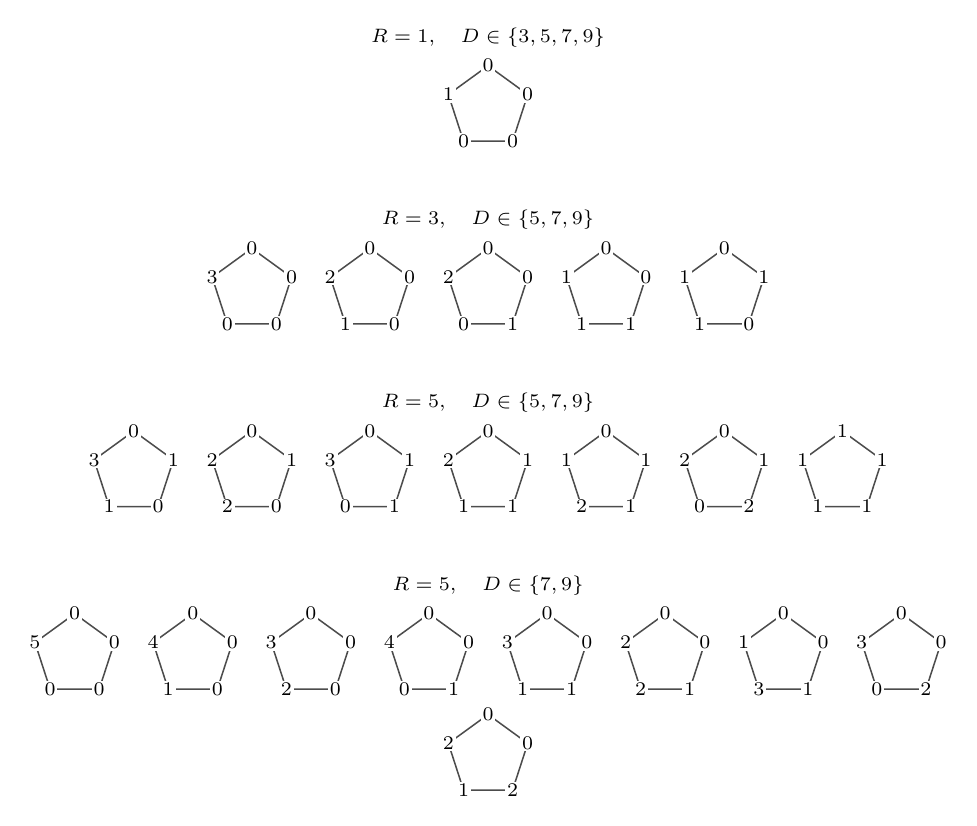
\begin{tikzpicture}[font=\scriptsize,
sc marked/.style={draw=red!65!black,line width=.75pt},
sc unmarked/.style={draw=blue!65!black,line width=.68pt,dash pattern=on 1.5pt off 1.35pt}]
\node[inner sep=0pt] at (0,0) {\(R=1,\quad D\in\{3,5,7,9\}\)};
\begin{scope}[shift={(0,-0.89)}]
\coordinate (c0) at (90:.53);
\coordinate (c1) at (18:.53);
\coordinate (c2) at (-54:.53);
\coordinate (c3) at (-126:.53);
\coordinate (c4) at (-198:.53);
\draw[black!70,line width=.55pt] (c0)--(c1)--(c2)--(c3)--(c4)--cycle;
\node[fill=white,inner sep=.65pt] at (c0) {\(0\)};
\node[fill=white,inner sep=.65pt] at (c1) {\(0\)};
\node[fill=white,inner sep=.65pt] at (c2) {\(0\)};
\node[fill=white,inner sep=.65pt] at (c3) {\(0\)};
\node[fill=white,inner sep=.65pt] at (c4) {\(1\)};
\end{scope}
\node[inner sep=0pt] at (0,-2.32) {\(R=3,\quad D\in\{5,7,9\}\)};
\begin{scope}[shift={(-3,-3.21)}]
\coordinate (c0) at (90:.53);
\coordinate (c1) at (18:.53);
\coordinate (c2) at (-54:.53);
\coordinate (c3) at (-126:.53);
\coordinate (c4) at (-198:.53);
\draw[black!70,line width=.55pt] (c0)--(c1)--(c2)--(c3)--(c4)--cycle;
\node[fill=white,inner sep=.65pt] at (c0) {\(0\)};
\node[fill=white,inner sep=.65pt] at (c1) {\(0\)};
\node[fill=white,inner sep=.65pt] at (c2) {\(0\)};
\node[fill=white,inner sep=.65pt] at (c3) {\(0\)};
\node[fill=white,inner sep=.65pt] at (c4) {\(3\)};
\end{scope}
\begin{scope}[shift={(-1.5,-3.21)}]
\coordinate (c0) at (90:.53);
\coordinate (c1) at (18:.53);
\coordinate (c2) at (-54:.53);
\coordinate (c3) at (-126:.53);
\coordinate (c4) at (-198:.53);
\draw[black!70,line width=.55pt] (c0)--(c1)--(c2)--(c3)--(c4)--cycle;
\node[fill=white,inner sep=.65pt] at (c0) {\(0\)};
\node[fill=white,inner sep=.65pt] at (c1) {\(0\)};
\node[fill=white,inner sep=.65pt] at (c2) {\(0\)};
\node[fill=white,inner sep=.65pt] at (c3) {\(1\)};
\node[fill=white,inner sep=.65pt] at (c4) {\(2\)};
\end{scope}
\begin{scope}[shift={(0,-3.21)}]
\coordinate (c0) at (90:.53);
\coordinate (c1) at (18:.53);
\coordinate (c2) at (-54:.53);
\coordinate (c3) at (-126:.53);
\coordinate (c4) at (-198:.53);
\draw[black!70,line width=.55pt] (c0)--(c1)--(c2)--(c3)--(c4)--cycle;
\node[fill=white,inner sep=.65pt] at (c0) {\(0\)};
\node[fill=white,inner sep=.65pt] at (c1) {\(0\)};
\node[fill=white,inner sep=.65pt] at (c2) {\(1\)};
\node[fill=white,inner sep=.65pt] at (c3) {\(0\)};
\node[fill=white,inner sep=.65pt] at (c4) {\(2\)};
\end{scope}
\begin{scope}[shift={(1.5,-3.21)}]
\coordinate (c0) at (90:.53);
\coordinate (c1) at (18:.53);
\coordinate (c2) at (-54:.53);
\coordinate (c3) at (-126:.53);
\coordinate (c4) at (-198:.53);
\draw[black!70,line width=.55pt] (c0)--(c1)--(c2)--(c3)--(c4)--cycle;
\node[fill=white,inner sep=.65pt] at (c0) {\(0\)};
\node[fill=white,inner sep=.65pt] at (c1) {\(0\)};
\node[fill=white,inner sep=.65pt] at (c2) {\(1\)};
\node[fill=white,inner sep=.65pt] at (c3) {\(1\)};
\node[fill=white,inner sep=.65pt] at (c4) {\(1\)};
\end{scope}
\begin{scope}[shift={(3,-3.21)}]
\coordinate (c0) at (90:.53);
\coordinate (c1) at (18:.53);
\coordinate (c2) at (-54:.53);
\coordinate (c3) at (-126:.53);
\coordinate (c4) at (-198:.53);
\draw[black!70,line width=.55pt] (c0)--(c1)--(c2)--(c3)--(c4)--cycle;
\node[fill=white,inner sep=.65pt] at (c0) {\(0\)};
\node[fill=white,inner sep=.65pt] at (c1) {\(1\)};
\node[fill=white,inner sep=.65pt] at (c2) {\(0\)};
\node[fill=white,inner sep=.65pt] at (c3) {\(1\)};
\node[fill=white,inner sep=.65pt] at (c4) {\(1\)};
\end{scope}
\node[inner sep=0pt] at (0,-4.64) {\(R=5,\quad D\in\{5,7,9\}\)};
\begin{scope}[shift={(-4.5,-5.53)}]
\coordinate (c0) at (90:.53);
\coordinate (c1) at (18:.53);
\coordinate (c2) at (-54:.53);
\coordinate (c3) at (-126:.53);
\coordinate (c4) at (-198:.53);
\draw[black!70,line width=.55pt] (c0)--(c1)--(c2)--(c3)--(c4)--cycle;
\node[fill=white,inner sep=.65pt] at (c0) {\(0\)};
\node[fill=white,inner sep=.65pt] at (c1) {\(1\)};
\node[fill=white,inner sep=.65pt] at (c2) {\(0\)};
\node[fill=white,inner sep=.65pt] at (c3) {\(1\)};
\node[fill=white,inner sep=.65pt] at (c4) {\(3\)};
\end{scope}
\begin{scope}[shift={(-3,-5.53)}]
\coordinate (c0) at (90:.53);
\coordinate (c1) at (18:.53);
\coordinate (c2) at (-54:.53);
\coordinate (c3) at (-126:.53);
\coordinate (c4) at (-198:.53);
\draw[black!70,line width=.55pt] (c0)--(c1)--(c2)--(c3)--(c4)--cycle;
\node[fill=white,inner sep=.65pt] at (c0) {\(0\)};
\node[fill=white,inner sep=.65pt] at (c1) {\(1\)};
\node[fill=white,inner sep=.65pt] at (c2) {\(0\)};
\node[fill=white,inner sep=.65pt] at (c3) {\(2\)};
\node[fill=white,inner sep=.65pt] at (c4) {\(2\)};
\end{scope}
\begin{scope}[shift={(-1.5,-5.53)}]
\coordinate (c0) at (90:.53);
\coordinate (c1) at (18:.53);
\coordinate (c2) at (-54:.53);
\coordinate (c3) at (-126:.53);
\coordinate (c4) at (-198:.53);
\draw[black!70,line width=.55pt] (c0)--(c1)--(c2)--(c3)--(c4)--cycle;
\node[fill=white,inner sep=.65pt] at (c0) {\(0\)};
\node[fill=white,inner sep=.65pt] at (c1) {\(1\)};
\node[fill=white,inner sep=.65pt] at (c2) {\(1\)};
\node[fill=white,inner sep=.65pt] at (c3) {\(0\)};
\node[fill=white,inner sep=.65pt] at (c4) {\(3\)};
\end{scope}
\begin{scope}[shift={(0,-5.53)}]
\coordinate (c0) at (90:.53);
\coordinate (c1) at (18:.53);
\coordinate (c2) at (-54:.53);
\coordinate (c3) at (-126:.53);
\coordinate (c4) at (-198:.53);
\draw[black!70,line width=.55pt] (c0)--(c1)--(c2)--(c3)--(c4)--cycle;
\node[fill=white,inner sep=.65pt] at (c0) {\(0\)};
\node[fill=white,inner sep=.65pt] at (c1) {\(1\)};
\node[fill=white,inner sep=.65pt] at (c2) {\(1\)};
\node[fill=white,inner sep=.65pt] at (c3) {\(1\)};
\node[fill=white,inner sep=.65pt] at (c4) {\(2\)};
\end{scope}
\begin{scope}[shift={(1.5,-5.53)}]
\coordinate (c0) at (90:.53);
\coordinate (c1) at (18:.53);
\coordinate (c2) at (-54:.53);
\coordinate (c3) at (-126:.53);
\coordinate (c4) at (-198:.53);
\draw[black!70,line width=.55pt] (c0)--(c1)--(c2)--(c3)--(c4)--cycle;
\node[fill=white,inner sep=.65pt] at (c0) {\(0\)};
\node[fill=white,inner sep=.65pt] at (c1) {\(1\)};
\node[fill=white,inner sep=.65pt] at (c2) {\(1\)};
\node[fill=white,inner sep=.65pt] at (c3) {\(2\)};
\node[fill=white,inner sep=.65pt] at (c4) {\(1\)};
\end{scope}
\begin{scope}[shift={(3,-5.53)}]
\coordinate (c0) at (90:.53);
\coordinate (c1) at (18:.53);
\coordinate (c2) at (-54:.53);
\coordinate (c3) at (-126:.53);
\coordinate (c4) at (-198:.53);
\draw[black!70,line width=.55pt] (c0)--(c1)--(c2)--(c3)--(c4)--cycle;
\node[fill=white,inner sep=.65pt] at (c0) {\(0\)};
\node[fill=white,inner sep=.65pt] at (c1) {\(1\)};
\node[fill=white,inner sep=.65pt] at (c2) {\(2\)};
\node[fill=white,inner sep=.65pt] at (c3) {\(0\)};
\node[fill=white,inner sep=.65pt] at (c4) {\(2\)};
\end{scope}
\begin{scope}[shift={(4.5,-5.53)}]
\coordinate (c0) at (90:.53);
\coordinate (c1) at (18:.53);
\coordinate (c2) at (-54:.53);
\coordinate (c3) at (-126:.53);
\coordinate (c4) at (-198:.53);
\draw[black!70,line width=.55pt] (c0)--(c1)--(c2)--(c3)--(c4)--cycle;
\node[fill=white,inner sep=.65pt] at (c0) {\(1\)};
\node[fill=white,inner sep=.65pt] at (c1) {\(1\)};
\node[fill=white,inner sep=.65pt] at (c2) {\(1\)};
\node[fill=white,inner sep=.65pt] at (c3) {\(1\)};
\node[fill=white,inner sep=.65pt] at (c4) {\(1\)};
\end{scope}
\node[inner sep=0pt] at (0,-6.96) {\(R=5,\quad D\in\{7,9\}\)};
\begin{scope}[shift={(-5.25,-7.85)}]
\coordinate (c0) at (90:.53);
\coordinate (c1) at (18:.53);
\coordinate (c2) at (-54:.53);
\coordinate (c3) at (-126:.53);
\coordinate (c4) at (-198:.53);
\draw[black!70,line width=.55pt] (c0)--(c1)--(c2)--(c3)--(c4)--cycle;
\node[fill=white,inner sep=.65pt] at (c0) {\(0\)};
\node[fill=white,inner sep=.65pt] at (c1) {\(0\)};
\node[fill=white,inner sep=.65pt] at (c2) {\(0\)};
\node[fill=white,inner sep=.65pt] at (c3) {\(0\)};
\node[fill=white,inner sep=.65pt] at (c4) {\(5\)};
\end{scope}
\begin{scope}[shift={(-3.75,-7.85)}]
\coordinate (c0) at (90:.53);
\coordinate (c1) at (18:.53);
\coordinate (c2) at (-54:.53);
\coordinate (c3) at (-126:.53);
\coordinate (c4) at (-198:.53);
\draw[black!70,line width=.55pt] (c0)--(c1)--(c2)--(c3)--(c4)--cycle;
\node[fill=white,inner sep=.65pt] at (c0) {\(0\)};
\node[fill=white,inner sep=.65pt] at (c1) {\(0\)};
\node[fill=white,inner sep=.65pt] at (c2) {\(0\)};
\node[fill=white,inner sep=.65pt] at (c3) {\(1\)};
\node[fill=white,inner sep=.65pt] at (c4) {\(4\)};
\end{scope}
\begin{scope}[shift={(-2.25,-7.85)}]
\coordinate (c0) at (90:.53);
\coordinate (c1) at (18:.53);
\coordinate (c2) at (-54:.53);
\coordinate (c3) at (-126:.53);
\coordinate (c4) at (-198:.53);
\draw[black!70,line width=.55pt] (c0)--(c1)--(c2)--(c3)--(c4)--cycle;
\node[fill=white,inner sep=.65pt] at (c0) {\(0\)};
\node[fill=white,inner sep=.65pt] at (c1) {\(0\)};
\node[fill=white,inner sep=.65pt] at (c2) {\(0\)};
\node[fill=white,inner sep=.65pt] at (c3) {\(2\)};
\node[fill=white,inner sep=.65pt] at (c4) {\(3\)};
\end{scope}
\begin{scope}[shift={(-0.75,-7.85)}]
\coordinate (c0) at (90:.53);
\coordinate (c1) at (18:.53);
\coordinate (c2) at (-54:.53);
\coordinate (c3) at (-126:.53);
\coordinate (c4) at (-198:.53);
\draw[black!70,line width=.55pt] (c0)--(c1)--(c2)--(c3)--(c4)--cycle;
\node[fill=white,inner sep=.65pt] at (c0) {\(0\)};
\node[fill=white,inner sep=.65pt] at (c1) {\(0\)};
\node[fill=white,inner sep=.65pt] at (c2) {\(1\)};
\node[fill=white,inner sep=.65pt] at (c3) {\(0\)};
\node[fill=white,inner sep=.65pt] at (c4) {\(4\)};
\end{scope}
\begin{scope}[shift={(0.75,-7.85)}]
\coordinate (c0) at (90:.53);
\coordinate (c1) at (18:.53);
\coordinate (c2) at (-54:.53);
\coordinate (c3) at (-126:.53);
\coordinate (c4) at (-198:.53);
\draw[black!70,line width=.55pt] (c0)--(c1)--(c2)--(c3)--(c4)--cycle;
\node[fill=white,inner sep=.65pt] at (c0) {\(0\)};
\node[fill=white,inner sep=.65pt] at (c1) {\(0\)};
\node[fill=white,inner sep=.65pt] at (c2) {\(1\)};
\node[fill=white,inner sep=.65pt] at (c3) {\(1\)};
\node[fill=white,inner sep=.65pt] at (c4) {\(3\)};
\end{scope}
\begin{scope}[shift={(2.25,-7.85)}]
\coordinate (c0) at (90:.53);
\coordinate (c1) at (18:.53);
\coordinate (c2) at (-54:.53);
\coordinate (c3) at (-126:.53);
\coordinate (c4) at (-198:.53);
\draw[black!70,line width=.55pt] (c0)--(c1)--(c2)--(c3)--(c4)--cycle;
\node[fill=white,inner sep=.65pt] at (c0) {\(0\)};
\node[fill=white,inner sep=.65pt] at (c1) {\(0\)};
\node[fill=white,inner sep=.65pt] at (c2) {\(1\)};
\node[fill=white,inner sep=.65pt] at (c3) {\(2\)};
\node[fill=white,inner sep=.65pt] at (c4) {\(2\)};
\end{scope}
\begin{scope}[shift={(3.75,-7.85)}]
\coordinate (c0) at (90:.53);
\coordinate (c1) at (18:.53);
\coordinate (c2) at (-54:.53);
\coordinate (c3) at (-126:.53);
\coordinate (c4) at (-198:.53);
\draw[black!70,line width=.55pt] (c0)--(c1)--(c2)--(c3)--(c4)--cycle;
\node[fill=white,inner sep=.65pt] at (c0) {\(0\)};
\node[fill=white,inner sep=.65pt] at (c1) {\(0\)};
\node[fill=white,inner sep=.65pt] at (c2) {\(1\)};
\node[fill=white,inner sep=.65pt] at (c3) {\(3\)};
\node[fill=white,inner sep=.65pt] at (c4) {\(1\)};
\end{scope}
\begin{scope}[shift={(5.25,-7.85)}]
\coordinate (c0) at (90:.53);
\coordinate (c1) at (18:.53);
\coordinate (c2) at (-54:.53);
\coordinate (c3) at (-126:.53);
\coordinate (c4) at (-198:.53);
\draw[black!70,line width=.55pt] (c0)--(c1)--(c2)--(c3)--(c4)--cycle;
\node[fill=white,inner sep=.65pt] at (c0) {\(0\)};
\node[fill=white,inner sep=.65pt] at (c1) {\(0\)};
\node[fill=white,inner sep=.65pt] at (c2) {\(2\)};
\node[fill=white,inner sep=.65pt] at (c3) {\(0\)};
\node[fill=white,inner sep=.65pt] at (c4) {\(3\)};
\end{scope}
\begin{scope}[shift={(0,-9.13)}]
\coordinate (c0) at (90:.53);
\coordinate (c1) at (18:.53);
\coordinate (c2) at (-54:.53);
\coordinate (c3) at (-126:.53);
\coordinate (c4) at (-198:.53);
\draw[black!70,line width=.55pt] (c0)--(c1)--(c2)--(c3)--(c4)--cycle;
\node[fill=white,inner sep=.65pt] at (c0) {\(0\)};
\node[fill=white,inner sep=.65pt] at (c1) {\(0\)};
\node[fill=white,inner sep=.65pt] at (c2) {\(2\)};
\node[fill=white,inner sep=.65pt] at (c3) {\(1\)};
\node[fill=white,inner sep=.65pt] at (c4) {\(2\)};
\end{scope}
\end{tikzpicture}
\caption{Five-cycle slack vectors with $R=1,3,5$. The five entries are read clockwise from the top. Each heading lists the degrees for which the vector satisfies the slack bound and all five parts are nonempty.}
\label{fig:finite-simple-slack-low}
\end{figure}
